\documentclass{article}
\usepackage{graphicx} % Required for inserting images
\usepackage[utf8]{inputenc}
\usepackage[T2A]{fontenc}
\usepackage{amsmath}
\usepackage{pgfplots}
\usepackage{longtable}
\usepackage{tabularx}
\usepackage{makecell}
\usepackage{array}
\usepackage{indentfirst}
\usepackage{icomma}
\usepackage{geometry}
\usepackage{booktabs}
\usepackage{multirow}
\usepackage{multicol}
\usepackage{float}
\usepackage{diagbox}
\usepackage{gensymb}
\geometry{a4paper, margin=1in}

\renewcommand{\figurename}{Изображение}
\renewcommand{\tablename}{Таблица}

\title{Лабораторная работа №2.03

Определение отношения теплоемкостей $ \frac{ C_{ p}}{ C_{ v}} $ методом звуковых стоячих волн}
\author{Топунов Антон, Z3142}
\date{14.02.2026}

\begin{document}

\maketitle
\clearpage
\section{Цели и задачи}
\subsection{Цели}
\begin{enumerate}
    \item Определение показателя адиабаты для воздуха при комнатной температуре.
\end{enumerate}
\subsection{Задачи}
\begin{enumerate}
    \item Прямое измерение координат пучностей (областей максимумов громкости звука) стоячей волны в трубке, частично заполненной водой.
    \item Обработка экспериментальных данных: получение скорости звука и соотношения теплоёмкостей.
\end{enumerate}
\section{Теоретическое введение}

Положение $i$-ой пучности:
\begin{gather*}
    X_{ i} = \frac{ 1}{ N}\sum\limits_{ j=1}^{ N}x_{ ij} 
\end{gather*}
\begin{itemize}
    \item $X_{ i}$ - средняя координата $i$-ой пучности.
    \item $x_{ ij}$ - $j$-е измерение координаты $i$-ой пучности.
    \item $N$ - количество измерений координаты каждой пучности. 
\end{itemize}

$l_{ i}$ - расстояние между положениями $i$-й и $i+1$-й пучностями:
\begin{gather*}
    l_{ i}=X_{ i+1} - X_{ i}
\end{gather*}

$l$ - среднее расстояние между пучностями:
\begin{gather*}
    l = \frac{ 1}{ M-1} \sum\limits_{ i=1}^{ M-1}l_{ i} \\
    \Delta l = t_{ \alpha ,  M-1}\cdot 
        \sqrt{\frac{ \sum\limits_{ i=1}^{M-1 }(l_{ i}-l)^2}{ (M-1)(M-2)} }
\end{gather*}
\begin{itemize}
    \item $M$ - количество точек , в которых измерялись положения пучностей.
    \item $\Delta l$ - погрешность расстояния между пучностями .
    \item $t_{ \alpha ,  M-1}$ - коэффициент Стьюдента .
\end{itemize}

$v$ - скорость звука в воздухе:
\begin{gather*}
    v= 2l\nu\\
    \Delta v = v \cdot \sqrt{\bigg( \frac{ \Delta{l}}{ l} \bigg)^2 + 
        \bigg( \frac{ \Delta{\nu}}{ \nu} \bigg)^2}
\end{gather*}
\begin{itemize}
    \item $\nu$ - частота генератора.
    \item $\Delta \nu$ - погрешность частоты генератора .
\end{itemize}

Абсолютная температура:
\begin{gather*}
    T = \,^{\circ}\text{t} - \,^{\circ}t_{ 0}\\
    \Delta T = \sqrt{(\Delta\,^{\circ}\text{t})^2+(\Delta\,^{\circ}\text{t}_{ 0})^2}
\end{gather*}
\begin{itemize}
    \item $^{\circ}\text{t}$ - температура в Цельсиях\\
    \item $^{\circ}t_{ 0}$ - точка абсолютного нуля в цельсиях\\
    \item $\Delta{^{\circ}\text{t}}$ и $\Delta{^{\circ}\text{t}_{ 0}}$ - их погрешности .    
\end{itemize}

Искомое отношение теплоёмкостей:
\begin{gather*}
    \frac{ C_{ p}}{ C_{ v}} = \frac{ v^2\mu}{ RT}\\
    \Delta \frac{ C_{ p}}{ C_{ v}} = \frac{ C_{ p}}{ C_{ v}} \cdot\sqrt{
        \bigg( \frac{ \Delta{R}}{ R} \bigg)^2 + \bigg( \frac{ \Delta{T}}{ T} \bigg)^2 +
        \bigg( \frac{ 2\Delta{v}}{ v} \bigg)^2 + \bigg( \frac{ \Delta{\mu}}{ \mu} \bigg)^2
    }
\end{gather*}
\begin{itemize}
    \item $R$ - универсальная газовая постоянная . 
    \item $T$ - абсолюная температура .
    \item $\mu$ - молярная масса воздуха . 
    \item $\Delta R$, $\Delta T$ , $\Delta \mu$ - их погрешности .
\end{itemize}

Теоретическое значение показателя адиабаты:
\begin{gather*}
    \frac{ C_{ p}}{ C_{ v}} = \frac{ i+2}{ i}
\end{gather*}
\begin{itemize}
    \item $i$ - количество степеней свободы воздуха.
\end{itemize}
\section{Схема установки}
Генератор (4) генерирует звуковую волну определённой частоты,
которая распространяется в сосуде (1).
Между его верхом и поверхностью воды создаётся стоячая волна.
С помощью наушника (5) можно улавливать уровень звука. Поднимая банку с водой (2) можно изменять уровень воды и искать области максимумов громкости звука.
С помощью линейки (6) положения точек максимума.  
\begin{figure}[H]
   \centering
   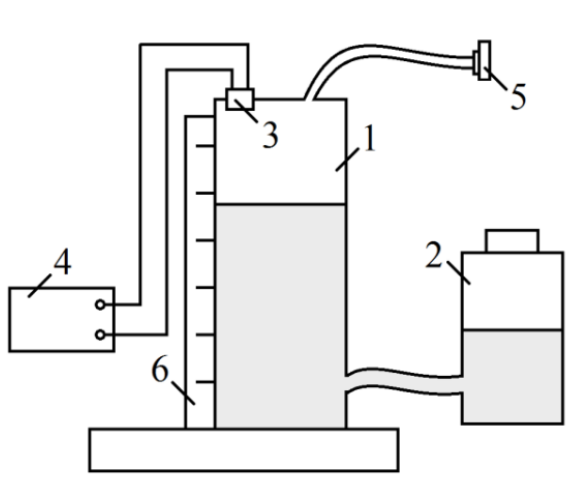
\includegraphics[width=0.8\linewidth]{sc.PNG}
   \caption{Схема установки}
\end{figure}
\section{Данные прямых измерений, табличные значения}
Количество пучностей:
\begin{gather*}
    M = 5
\end{gather*}
Количество измерений в каждой пучности:
\begin{gather*}
    N = 5
\end{gather*}
Коэффициент Стьюдента:
\begin{gather*}
    t_{ 0.95 , 4} = 3.18
\end{gather*}
Частота генератора:
\begin{gather*}
    \nu=1.5 \text{ ГГерц}\\
    \Delta \nu=0.05 \text{ ГГерц}\\
\end{gather*}
Температура:
\begin{gather*}
    ^{\circ}t = 22 \text{ } ^{\circ}\text{C}\\
    \Delta ^{\circ}t = 1 \text{ } ^{\circ}\text{C} \\
    ^{\circ}t_{ 0} = -273 \text{ } ^{\circ}\text{C}\\
    \Delta ^{\circ}t_{ 0} = 0.5 \text{ } ^{\circ}\text{C}
\end{gather*}

Универсальная газовая постоянная 
\begin{gather*}
    R = 8.31 \, \frac{ \text{Дж}}{ \text{К}\cdot\text{моль}}\\
    \Delta R = 0.005 \, \frac{ \text{Дж}}{ \text{К}\cdot\text{моль}}
\end{gather*}

Молярная масса воздуха 
\begin{gather*}
    \mu = 29 \,\frac{ \text{г}}{ \text{моль}}\\
    \mu = 0.5 \,\frac{ \text{г}}{ \text{моль}}
\end{gather*}

\begin{table}[H]
   \centering
   \begin{tabular}{|c|c|c|c|c|c|} \hline
$j$ & $1$ & $2$ & $3$ & $4$ & $5$\\\hline
$x_{1j}$, мм & $110$ & $114$ & $112$ & $115$ & $116$\\\hline
$x_{2j}$, мм & $230$ & $226$ & $228$ & $231$ & $225$\\\hline
$x_{3j}$, мм & $349$ & $345$ & $348$ & $347$ & $347$\\\hline
$x_{4j}$, мм & $462$ & $467$ & $466$ & $463$ & $466$\\\hline
$x_{5j}$, мм & $574$ & $584$ & $582$ & $583$ & $584$\\\hline
   \end{tabular}
   \caption{Результаты измерений коорддинат пучностей}
\end{table}

\section{Расчёты и графики}

Вычисленные средние значения координат и соответствующие расстояния между ними:
\begin{table}[H]
   \centering
   \begin{tabular}{|c|c|c|c|c|c|} \hline
$i$ & $X_{i}$, мм & $l_{i}$, мм \\\hline
$1$ & $113.4$ & $114.6$\\\hline
$2$ & $228.0$ & $119.2$\\\hline
$3$ & $347.2$ & $117.6$\\\hline
$4$ & $464.8$ & $116.6$\\\hline
$5$ & $581.4$ & \\\hline
   \end{tabular}
   \caption{Вычисленные значения}
\end{table}

Примеры вычислений:
\begin{gather*}
X_1 = \dfrac{110 + 114 + 112 + 115 + 116}{5}\approx113.4\text{ мм}\\
l_1 = 228 - 113.4 \approx114.6\text{ мм}\\
\end{gather*}

Среднее значение расстояния между пучностями и погрешность разброса:
\begin{gather*}
    l = \frac{ 114.6+119.2+117.6+116.6}{ 4}\approx117.0\text{ мм}\\
    \Delta l = 3.18 \cdot \sqrt{\frac{ (114.6-117.0)^2+(119.2-117.0)^2+(117.6-117.0)^2+(116.6-117.0)^2}{ 4\cdot3} }\approx3.1 \text{ мм}
\end{gather*}

Скорость звука в воздухе:
\begin{gather*}
    v= 2 \cdot 117.0 \cdot 1.5 \approx 351 \, \frac{ \text{м}}{ \text{с}}\\
    \Delta v = 351\cdot \sqrt{\bigg( \frac{ 3.1}{ 117.0}\bigg)^2 +
        \bigg( \frac{ 0.05}{ 1.5}\bigg)^2} \approx 15 \, \frac{ \text{м}}{ \text{с}}
\end{gather*}

Абсолютная температура:
\begin{gather*}
    T = 22 + 273 = 295 \text{ К}\\
    \Delta T = \sqrt{(1)^2+(0.5)^2} \approx 1.1 \text{ К}
\end{gather*}

Искомый показатель адиабаты:
\begin{gather*}
    \frac{ C_p}{ C_v} = \frac{ 351^2\cdot0.029}{ 8.31\cdot295}\approx 1.46\\
    \Delta \frac{ C_{ p}}{ C_{ v}} = 1.46 \cdot\sqrt{
        \bigg( \frac{ 0.005}{ 8.31} \bigg)^2 + \bigg( \frac{ 1.1}{ 295} \bigg)^2 +
        \bigg( \frac{ 2\cdot15}{ 351} \bigg)^2 + \bigg( \frac{ 0.5}{ 29} \bigg)^2 
    } \approx 0.13
\end{gather*}

Теоретическое значение:
\begin{gather*}
    \frac{ C_p}{ C_v} = \frac{ 5+2}{ 5}=1.4
\end{gather*}
\section{Результаты и выводы}
Значение показателя адиабаты, с учётом погрешности $\frac{ C_p}{ C_v}=1.46\pm0.13$ совпадает с реальным показателем адиабаты воздуха $\frac{ C_p}{ C_v}=1.4$.
Полученная скорость звука $v = (351\pm15)\,\frac{ \text{м}}{ \text{с}}$ совпадает с скоростью звука при адиабатическом процессе ($v\approx344 \,\frac{ \text{м}}{ \text{с}}$).
Относительные погрешности не очень велики ($\varepsilon_{ v} \approx 4.3$, $\varepsilon_{ \frac{ C_p}{C_v } } \approx 8.9 \%$). Это показывает что эксперимент был проведён с достаточной точностью и адиабатическое приближение к распространению звуковых волн можно считать верным.

\clearpage

\begin{figure}[H]
   \centering
   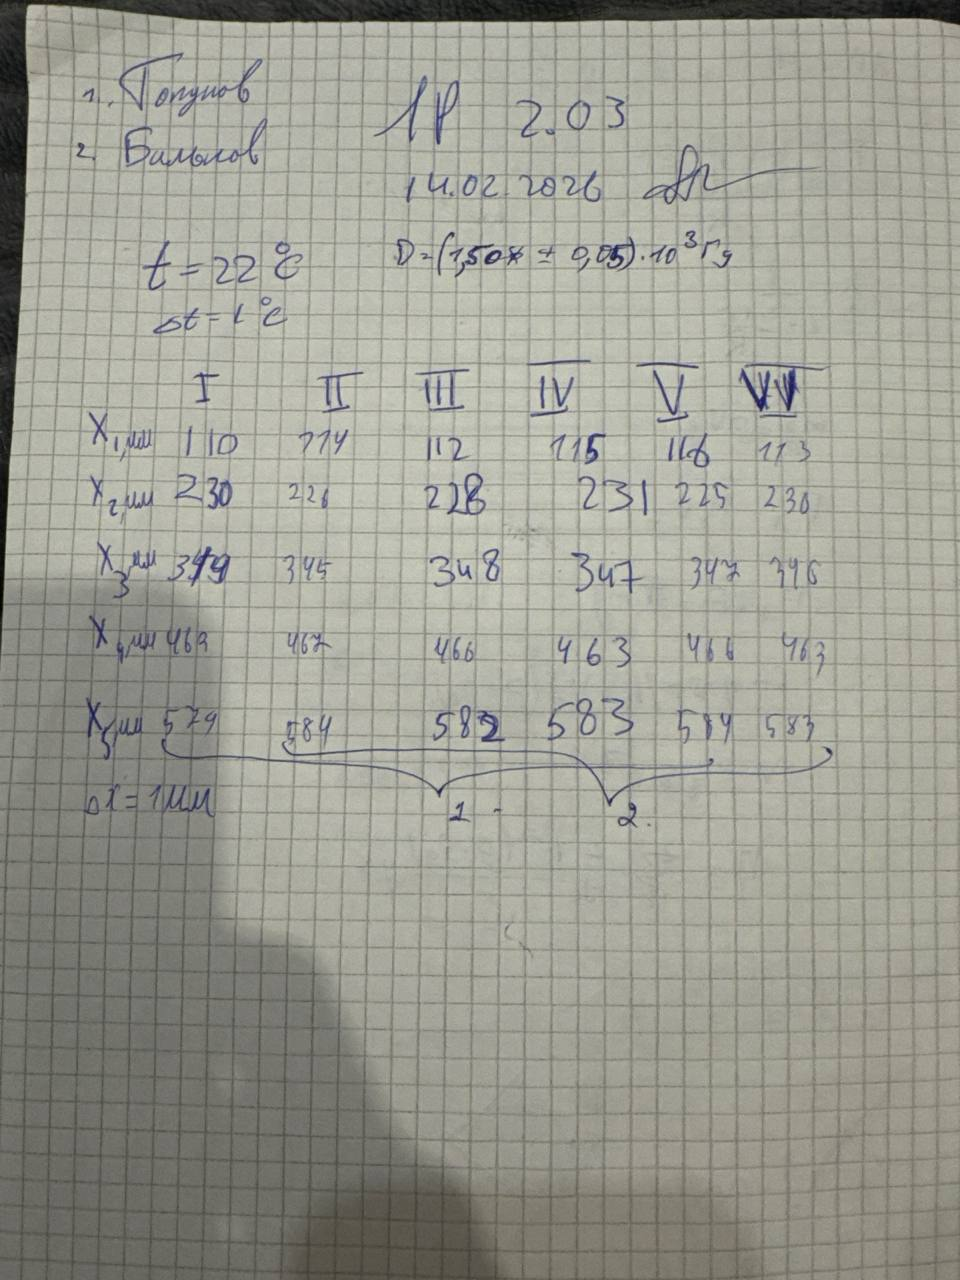
\includegraphics[width=0.8\linewidth]{23599.jpg}
   \caption{Подписанне пряме измерения}
\end{figure}
\end{document}